%!TEX root = ../dokumentation.tex
\chapter{Planung und Konzeption}
In diesem Kapitel werden die Anforderungen für ein digitales Funkübertragungssystem definiert, welches die Möglichkeit bieten soll beliebige Signale im Bereich der Dezimeterwelle zu analysieren und zu verarbeiten. Das aus dieser Definition resultierende System wird im Verlauf dieses Kapitels geplant und implementiert.\\
Um möglichst viele Dienste im Frequenzbereich der Dezimeterwelle analysieren zu können sollte der Hardwareaufbau, bestehend aus Antenne und digitalem Empfängersystem, folgende Eigenschaften besitzen:
\begin{itemize}
	\item Die Antenne sollte möglichst breitbandig sein. Sie muss mindestens den vorgegeben Bereich zwischen 300 MHz und 3000 MHz abdecken.
	\item Um ein Signal vollständig zu erfassen muss auch das digitale Empfängersystem eine ausreichende Kanalbandbreite aufweisen.
	\item Die Abtastrate des Systems muss gemäß Abschnitt \ref{abtasttheorem} ausreichend hoch sein um das Signal rekonstruieren zu können.
	\item Das System muss mit einem Unix-ähnlichem Betriebssystem oder mit Microsoft Windows bedienbar sein.
	\item Der Dynamikumfang des Systems muss ausreichend groß sein. Das bedeutet, dass das Differenz zwischen dem größtmöglichen zum kleinstmöglichen Pegel im Verhältnis zueinander stehen muss. Der grobe Richtwert von 40 dB liegt der Unterschied zwischen den Werten bei 1:10 000. Dabei ist die untere Grenze erfassbarer Signale das Grundrauschen im System und dessen Umgebung; der Bereich nach oben wird hingegen durch die maximal erfassbare Signalgröße eingeschränkt.
	\item Das System soll unter wirtschaftlichem Gesichtspunkt entworfen werden. Bedeutet ausreichende Funktionen unter Betrachtung der preislichen Situation.
\end{itemize}

Die aufgeführten Anforderungen werden bei der Planung des Systems, besonders bei der Auswahl der Hardware, berücksichtigt. Auf den folgenden Seiten wird auf die einzelnen Punkte näher eingegangen. 

Zunächst wird jedoch im Verlauf des Kapitels das Frequenzspektrum der Dezimeterwelle und die rechtlichen Rahmenbedingungen für Dienste in diesem Bereich untersucht, um mögliche Rückschlüsse auf das zu entwerfende System ziehen zu können.


\newpage
\section{Das Frequenzspektrum}
\label{section-frequenzbereiche}
Zur Orientierung im Spektrum elektromagnetischer Wellen haben sich international verschiedene Systeme zur Klassifikation sogenannter Frequenzbänder gebildet. Die \ac{ITU} empfiehlt eine Einteilung des Spektrums von 3 kHz bis 300 GHz in acht Frequenzbereiche, auch Frequenzdekaden genannt. \cite[vgl. ITU-R v.431-8]{itu-431:2015}

\begin{figure}[ht]
	\centering
	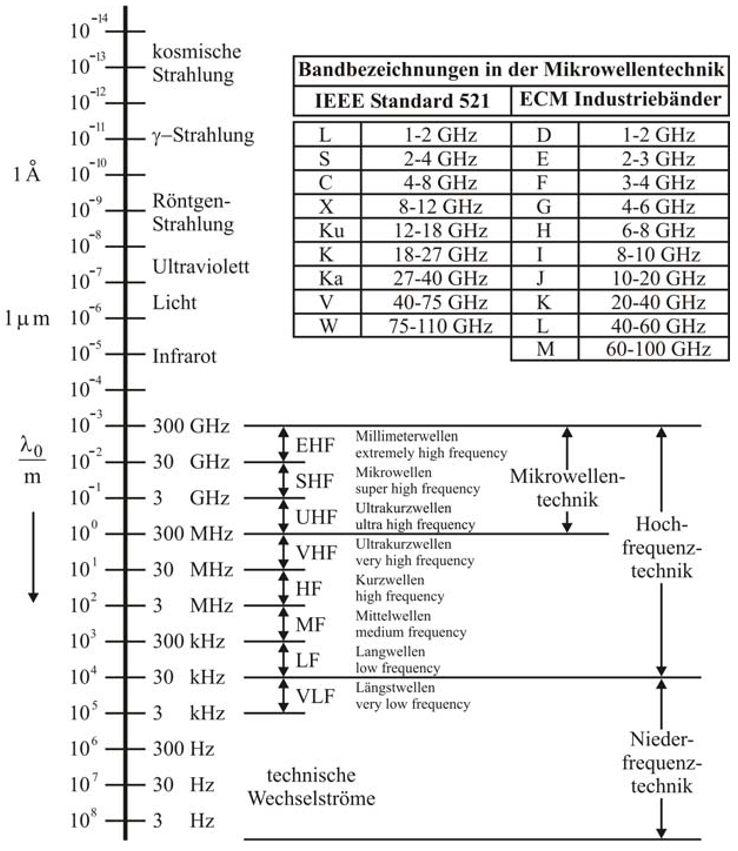
\includegraphics[width=0.75\textwidth]{frequenzbereich.png}
	\caption[Spektrum elektromagnetischer Wellen und gebräuchliche Bandbezeichnungen]{Spektrum elektromagnetischer Wellen und gebräuchliche Bandbezeichnungen. Quelle: \cite[Kark, S. 1]{Kark:2017}} 
	\label{frequenzbereiche}
\end{figure}




\subsection{Rechtliche Grundlagen}
In Deutschland gilt rechtlich zudem die Aufteilung des Frequenzbereiches von 9 kHz bis 3000 GHz, welche von der Bundesnetzagentur im sogenannten Frequenzplan \cite[Bundesnetzagentur, 2016]{bundesnetzagentur-frequenzplan:2016} gemäß § 54 TKG festgehalten wird.
Dort werden die Frequenzbereiche nach Frequenznutzung (Amateurfunk, Seefunk, WLAN, etc.) eingeteilt und entsprechende Nutzungsbestimmungen spezifiziert:

\begin{figure}[ht]
	\centering
	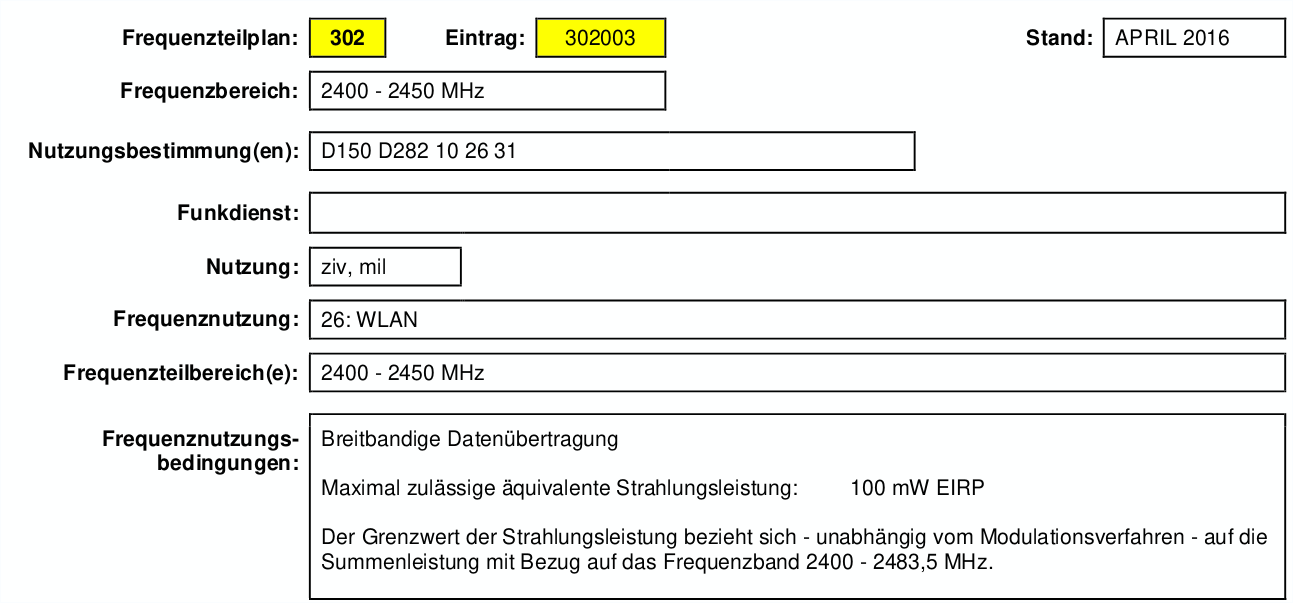
\includegraphics[width=\textwidth]{freqplan-wlan.png}
	\caption[Eintrag: 2,4 GHz WLAN im Frequenzplan]{Eintrag: 2,4 GHz WLAN im Frequenzplan. Quelle: \cite[Bundesnetzagentur, 2016]{bundesnetzagentur-frequenzplan:2016}}
	\label{frequenzplan-wlan}
\end{figure}


\section{Anwendungen im Bereich der Dezimeterwelle}
Das Frequenzband von 300 MHz bis 3 GHz, auch \ac{UHF}-Band genannt, ist ein Frequenzbereich in dem die Wellen eine Länge von zehn Dezimeter bis einem Dezimeter besitzen:
\( \lambda = \frac{c}{f} = \frac{3*10^8 \text{ m/s}}{300 \text{ MHz}} = 1\text{ m}\)
und
\( \frac{3*10^8 \text{ m/s}}{3000 \text{ MHz}} = 0.1\text{ m}\).
Der damit untersuchte Frequenzbereich erstreckt sich von 300 MHz bis 3 GHz. Darunter befinden sich die gängigsten Anwendungen, die im folgenden detaillierte beschrieben werden.

In dem oben genannten Frequenzbereich liegen unter anderem folgende Anwendungen:

\begin{description}
	\item [\ac{GSM} 400]{In diesem Frequenzbereich von 380 Mhz - 496 MHz befindet sich der digitale \ac{BOS}-Funk. Der BOS-Funk ist ein nichtöffentlicher mobiler \ac{UKW}-Funkdienst. Über diese Technik können Einsatzkräfte miteinander kommunizieren oder direkt alarmiert werden.}
	\item [\ac{SRD}] {Short Range Devices sind Funkanwendungen die Jedermann für Sprach und Datenübertragung verwenden kann. Darunter liegen Geräte wie der Autoschlüssel, Wetterstationen und weitere Anwendungen im Smart Home Bereich. Diese Funktechnik liegt im Bereich von 443 MHz. Um in Zukunft die Störung innerhalb dieser Technik zu verringern  wurde das 860 Mhz-Band festgelegt. Dieses wurde in mehrere Subbänder unterteilt, um gegenseitige Störungen zu vermeiden. Dieser Bereich erstreckt sich von 863 MHz - 870 MHz. Jedes dieser Subbänder hat für die Nutzung besondere Parameter vorgesehen. Darunter kommunizieren Geräte wie Funk-Alarmanlagen und gewisse "Internet of Things"- Geräte.}
	\item [\ac{GSM} 900] {GSM ist ein Mobilfunkstandard für Mobilfunknetze. Hauptsächlich wird dieses Netz für Telefonie und Datenübertragung wie Kurzmitteilungen (SMS). GSM wurde als mobile Alternative zum ISDN Telefonnetz entwickelt. Das GSM Netz bietet die technische Grundlage der D- und E-Netze.  }
	\item [\ac{GPS}] {Das GPS ist ein globales Navigationssatellitensystem zur Positionsbestimmung. Die Kommunikation der spezifischen Daten wie Position und Uhrzeit erfolgt auf der Frequenz 1227,60 Mhz. Zur genauen Positionsbestimmung muss ein Empfänger die Signale von vier Satelliten gleichzeitig empfangen. Im Empfangsgerät werden die Signallaufzeiten gemessen und unter Berücksichtigung der Uhrfehler, die aktuelle Position und Höhe errechnet.}
	\item [\ac{DECT}] {DECT ist ein internationaler Standard für Telekommunikation mittels Funktechnik häufig bei Mobiltelefonen. Dieser Standard arbeitet grundsätzlich verbindungsorientiert und ist primär für Telefonie innerhalb von Gebäuden ausgelegt. Deren Reichweite beträgt ca. 30-50 Meter. DECT beschreibt eine reine Zugangstechnologie im Gegensatz zu herkömmlichen Mobilfunksystemen. Der Frequenzbereich bei DECT liegt bei 1880 MHz-1900 MHz.}
	\item [\ac{ISM}] {ISM bezeichnet die Hochfrequenz-Geräte, die für Industrie, Wissenschaft, Medizin und häuslichen Bereichen eingesetzt werden. Die bekanntesten Anwendungen darunter sind  WLAN und Bluetooth.}
\end{description}


\section{Software}
\subsection{SDR Sharp}
SDR\# (gesprochen: \enquote{SDR Sharp}) ist eine kostenlose Software von Airspy \cite{airspy:2018}, die ausschließlich für Microsoft Windows erhältlich ist. Mit dieser Anwendung lassen sich u. a. mittels Software Defined Radio Systemen empfangene Signale auslesen und etwa im Frequenzbereich oder in einem Wasserfalldiagramm visualisieren.
So lassen sich einige Modulationsarten relativ schnell testen. 

In der Abbildung \ref{SDRSharp}  ist die Oberfläche von SDR\# zu erkennen. Im oben drittel des Bereichs ist das erkannte Signal dargestellt. Auf der linken Seite können unterschiedliche Einstellung vorgenommen werden. Eine essenzielle Eigenschaft ist das einstellen der Modulationsart. Damit kann sehr leicht getestet werden, ob bei dem empfangenen Signal es sich um eine Frequenzmodulation oder Amplitudenmodulation handelt. Im unteren rechten Bereich wird ein Fenster angezeigt, das den Namen Audio Spektrum trägt. In der Abbildung ist ein Audio Spektrum zu erkennen, was bedeutet, dass etwas zu hören ist. Im Gegensatz zu der Amplitudenmodulation wird in diesem Fenster somit gar nichts angezeigt. Somit kann durch eine Aufnahme des Signals mit unterschiedlichen Modulationsarten getestet werden, wie das Signal aufgebaut wird und dekodiert werden kann.

\begin{figure}[H]
	\centering
	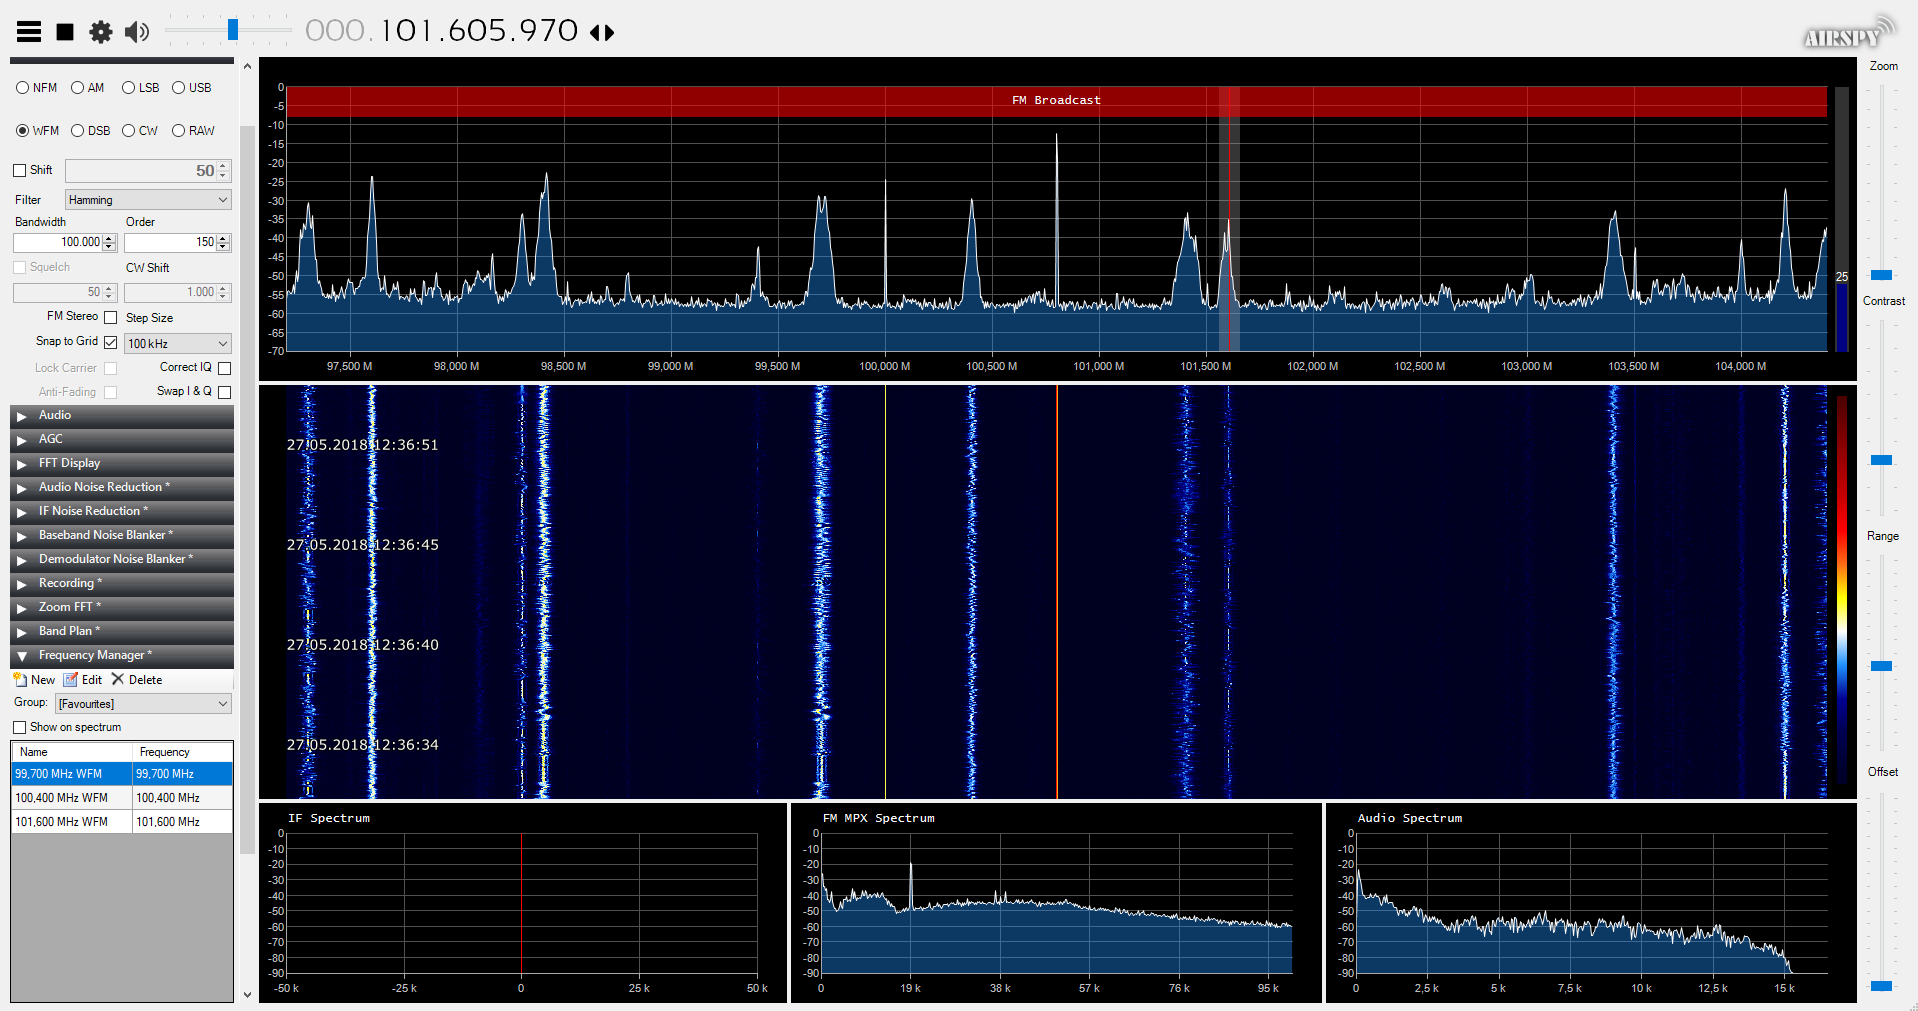
\includegraphics[width=1.0\textwidth]{SdrSharp.png}
	\caption[SDR Sharp: Modulationsartbestimmung an einem konkreten Beispiel]{SDR Sharp: Modulationsartbestimmung an einem konkreten Beispiel} 
	\label{SDRSharp}
\end{figure}


\subsection{GNU Radio}
GNU Radio \cite{gnuradio} ist ein freies, quelloffenes Entwicklerwerkzeug zur Implementierung von Software Defined Radio mittels Signalverarbeitungsblöcken. Es kann mit externer Funkhardware oder als Simulation ohne zusätzliche Hardware genutzt werden. GNU Radio ist im Hobbybereich weit verbreitet, wird aber auch in der Wissenschaft und im kommerziellen Bereich genutzt. GNU Radio Programme können zusätzlich durch selbst programmierte Ergänzungsblöcke erweitert werden. Die können wahlweise in den Programmiersprachen Python oder C++ geschrieben werden, wobei sich besonders für echtzeitkritische Signalverarbeitungen letzteres anbietet.\\
GNU Radio bietet zusätzlich eine grafische Oberfläche mit \ac{GRC}, die es ermöglicht Blockschaltbilder als Flowgraph darzustellen.

\subsubsection{Funktionsweise}
GNU Radio verarbeitet den Datenstrom, der vom Empfänger kommt, oder bereitet Daten vor, um diese zu senden. Dabei ist die gesamte Datenverarbeitung in Blöcke eingeteilt, die  beliebig  zusammengestellt  werden können. GNU Radio liefert eine Vielzahl von Filtern, Kanal-Codes, Synchronisationselementen, Equalizern, Demodulatoren, und weitere gängige Werkzeuge der Nachrichten- und Funktechnik. Diese Blöcke stellen die Hardwarekomponenten klassischer Funkhardware dar. Falls nötig können auch selbst Blöcke hinzugefügt werden. Dabei sollte darauf geachtet werden, dass ein Block genau eine Aufgabe erledigt, damit er so vielseitig wie möglich eingesetzt werden kann. GNU Radio bietet die Möglichkeit, diese Blöcke miteinander zu verbinden und regelt dadurch den Datenfluss zwischen verbundenen Blöcken. \\

Für die digitale Verarbeitung von Daten kommen in GNU Radio verschiedene Datentypen zum Einsatz: Der Datenstrom des Empfängers besteht in den meisten Fällen aus komplexen Zahlen, also einem Datentyp, bei dem jedes Datum aus zwei Float-Werten, dem Imaginärteil und dem Realteil, besteht (siehe Abschnitt \ref{iq}). \\
Als Ein- oder Ausgänge eines Blocks können jedoch verschiedene Datentypen zum Einsatz kommen, üblicherweise Short, Byte, Integer und Float. Der Datentyp am Eingang und Ausgang eines Blockes muss dabei nicht gleich sein.\\

Um mit GNU Radio eine SDR-Anwendung zu erstellen, muss man Blöcke, die die einzelnen Funktionseinheiten darstellen, miteinander zu einem Graphen kombinieren. Sollte ein benötigter Block nicht verfügbar sein, kann man diesen mittels einem Tool selbst hinzufügen. Beim Starten des Graphen ruft GNU Radio nun jeden Block nacheinander auf und stellt sicher, dass Daten von einem Block zum Nächsten weitergereicht werden. Ergebnisse  können  durch  Graphical  User  Interface  (GUI)-Blöcke dargestellt werden. Diese nutzen die freien und plattformübergreifenden GUI-Toolkits.


\section{Hardware}

\subsection{Antenne} 

Ganz allgemein kann man Antennen als Koppelelemente zwischen geführten und ungeführten elektromagnetischen Wellen, d. h. als Wandler zwischen Leitungs- und Freiraumwellen, auffassen. Quelle ist immer ein elektrischer oder magnetischer Dipol. Durch eine (Raum-)Transformation im Nahbereich, bei der die Richtungen der Felder (innerhalb der Fortpflanzungsgeschwindigkeit) gedreht werden, entsteht im Fernbereich die gelöste Wellenfront einer elektromagnetischen Welle. 

Elektromagnetische Wellen bestehen aus polarisierten elektrischen und magnetischen Feldern, die sich durch Kopplung wechselseitig erzeugen und im Vakuum ohne Verluste als Transversalwellen räumlich ausbreiten. Bei vorgegebenen Randbedingungen liefern die Maxwellschen Gleichungen eine exakte Beschreibung. In der Praxis berechnet man die Abstrahlung der Energie aber meist durch Näherungsverfahren. 

Eine Antenne die aus der Aufgabenstellung hervorgeht, muss dementsprechend den Frequenzbereich der Dezimeterwelle abdecken. Grundsätzlich gibt es zwei Möglichkeiten ein solches Analysesystem zu betreiben: Mit stationärer oder mobiler Antenne.

Eine mobile Antennenlösung, die den oben genannten Anforderung gerecht wird wäre die HyperLOG 4040 Antenne. Sie ist eine Logarithmisch Periodische Breitband Antenne. Eine LPDA besteht aus einer Anzahl von Dipolantennen, deren Länge und Abstand zur Strahlungsrichtung hin abnehmen. Ein großer Vorteil dieser Technik ist die hohe Bandbreite der Antenne. Damit deckt Sie den Frequenzbereich der Aufgabe ab. Ein massiver Nachteil dieser Antennenart ist die Richtwirkung, dabei empfängt diese Arte der Antenne die Signale besser, wenn Sie zum Signal ausgerichtet wird. Ein weiterer negativer Faktor sind die enormen Kosten. Mit ca 350\euro ist diese Antenne in der oberen Preisregion angesiedelt. In der nachfolgenden Tabelle sind die technischen Daten der Antenne zu erkennen. 

\begin{figure}[H]
	\centering
	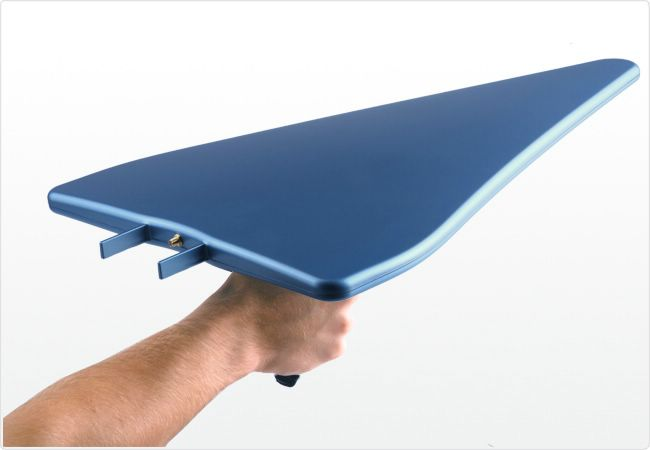
\includegraphics[width=0.5\textwidth]{logper_antenne_hyperlog404.png}
	\caption[HyperLOG 4040]{HyperLOG 4040. Quelle: \cite{Funktechnik:2018}} 
	\label{HyperLOG 4040}
\end{figure}  

Die im folgenden gezeigte Tabelle beschreibt die technischen Daten der HyperLOG 4040 Antenne. Somit kann Sie auf einen Blick mit der im nachfolgenden evaluierten Antenne verglichen werden.

\begin{table}[H]
	\centering
	\begin{tabular}{c|c}
		Modell & HyperLOG 4040\\
		\hline
		Antennentyp & Logarithmisch Periodische Breitband Antenne\\ 
		\hline 
		Bandbreite & 400 MHz - 4 GHz\\ 
		\hline 
		Länge &  60 cm\\ 
		\hline 
		Preis in \euro &  350 \euro \\ 
		\hline 
		Installationsart & Mobil\\ 
		
	\end{tabular} 
	\caption{Produktinformationen der HyperLOG 4040 Antenne}
\end{table}

Die Sirio SD 3000N ist eine stationäre Lösungsmöglichkeit, welche den zuvor genannten Anforderungen gerecht wird. Diese Antenne wird als eine Discone-Antenne bezeichnet. Ihr Vorteil besteht aus Ihrem Aufbau, sie wird auch als breitbandige Rundstrahlantenne bezeichnet. Ihr wesentlicher Vorteil liegt im niedrigen Abstrahlwinkel und die Grenzfrequenzen werden durch die Abmessungen der Antenne begrenzt. Durch Ihre Breitbandigkeit wird die Discone-Antenne häufig für Funküberwachungsaufgaben verwendet. Im Gegensatz zu der LPDA ist die Wirkrichtung des Signal bei dieser Technik nicht von Nöten. Da diese Antenne bei einer preislichen Budget von 90 \euro liegt ist sie deutlich günstiger und reicht für die genannten Anforderung vollkommen aus.


\begin{figure}[H]
	\centering
	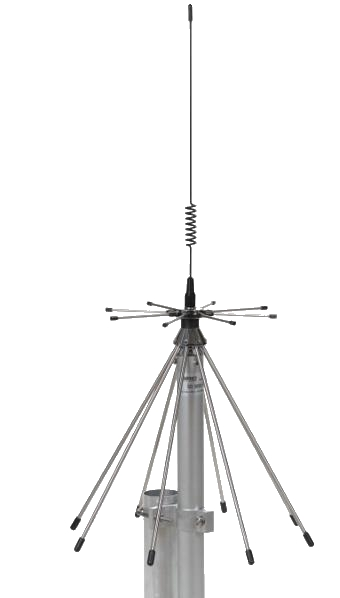
\includegraphics[width=0.4\textwidth]{SirioSD3000N.png}
	\caption[Sirio SD 3000N stationäre Funkantenne]{Sirio SD 3000N stationäre Funkantenne. Quelle: \cite{Funktechnik:2018}} 
	\label{Sirio SD 3000N Antenne}
\end{figure}

Im Folgenden Abschnitt beschreibt eine Tabelle die technischen Daten der Sirio SD 3000N. Damit die Antennenmöglichkeiten miteinander verglichen werden könnnen um ein abschließendes Resümee gezogen werden kann. Durch die oben genannten Vorteile der Sirio SD 3000N gegenüber der HyperLOG 4040 spricht das Ergebnis für Sie. 

\begin{table}[H]
	\centering
	\begin{tabular}{c|c}
		Modell & Sirio SD 3000N\\
		\hline
		Antennentyp & Discone Antenne\\ 
		\hline 
		Bandbreite & 300 MHz - 3 GHz\\ 
		\hline 
		Länge &  72 cm\\ 
		\hline 
		Preis in \euro &  90 \euro \\ 
		\hline 
		Installationsart & Stationär\\ 
		
	\end{tabular} 
	\caption{Produktinformationen der Sirio SD 3000N Antenne}
\end{table}


\subsection{SDR-Gerät} 
Ein Software Defined Radio Gerät, das man experimentell betreiben kann, reicht von mehreren tausend Euro teuren Forschungsgeräte bis zu kostenlosen Geräten, da selbst mittels einem Mikrofoneingang der Soundkarte am Computers, manche Signale empfangen werden können. Die Geräte unterscheiden sich hauptsächlich in Fähigkeiten wie:

\begin{itemize}
	\item Frequenzbereich
	\item maximale Bandbreite
	\item Abtastrate
\end{itemize}

Beim Computer kommen häufig Universal Serial Bus (USB) und Ethernet als Schnittstelle zum  Einsatz.
Da nur Empfängersignale betrachtet werden sollen, würde ein handelsüblicher DVB-T-Stick eine günstige Option darstellen. Mithilfe des entsprechenden Treibers kann der Stick mit GNU Radio genutzt werden, jedoch deckt sich der Frequenzbereich des Gerätes nicht, mit dem innerhalb der Aufgabenstellung beschriebenen Dezimeterwelle.\\

\begin{figure}[H]
	\centering
	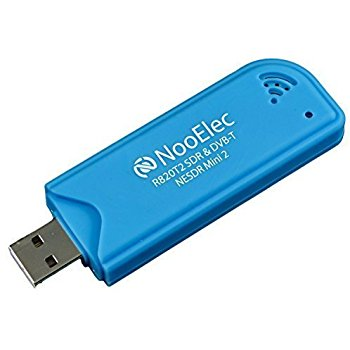
\includegraphics[width=0.5\textwidth]{NooElec.png}
	\caption[NooElec DVB-T Stick]{NooElec DVB-T Sick. Quelle: \cite{NooElec:2018}} 
	\label{NooElec}
\end{figure}

Das SDR-Gerät muss in Kombination mit der Funkantenne über den kompletten Frequenzbereich der Dezimeterwelle erstrecken, um die Metainformationen in diesem Bereich zu analysieren. Aus diesem Grund kann ein solchen Gerät für diese Arbeit nicht verwendet werden. Aus der Tabelle können die groben Daten des DVB-T Sticks entnommen werden.\\

\begin{table}[h]
	\centering
	\begin{tabular}{c|c}
		Modellbezeichnung & RTL2832U\\
		\hline
		Hersteller & NooElec\\ 
		\hline 
		Frequenzbereich & 25 MHz - 1750 MHz \\ 
		\hline 
		Preis in \euro & 20 \euro \\ 
		\hline 
		Installationsart & Mobil \\ 
		\hline 
		RX/TX & RX Receiver \\ 
	\end{tabular} 
	\caption{Produktinformationen des NooElec RTL2832U}
\end{table}

Ein gutes Preis-Leistungsverhältnis bietet das HackRF One Board \cite{greatscott}. Die HackRF One Platine ist ein flexibles Testmodul für die Funkmesstechnik, das wie ein Software Defined Radio (SDR) arbeitet. Sie ist ein Open Source Hardware Transceiver, der hauptsächlich zu eigenen Versuchen und Messungen für SDRs eignet, außerdem ist dieses Gerät für die HF-Technik und messtechnischen Versuchsaufbauten im Amateurfunk vergleichsweise geringen Preises von rund 300 Euro sehr beliebt.\\

\begin{figure}[H]
	\centering
	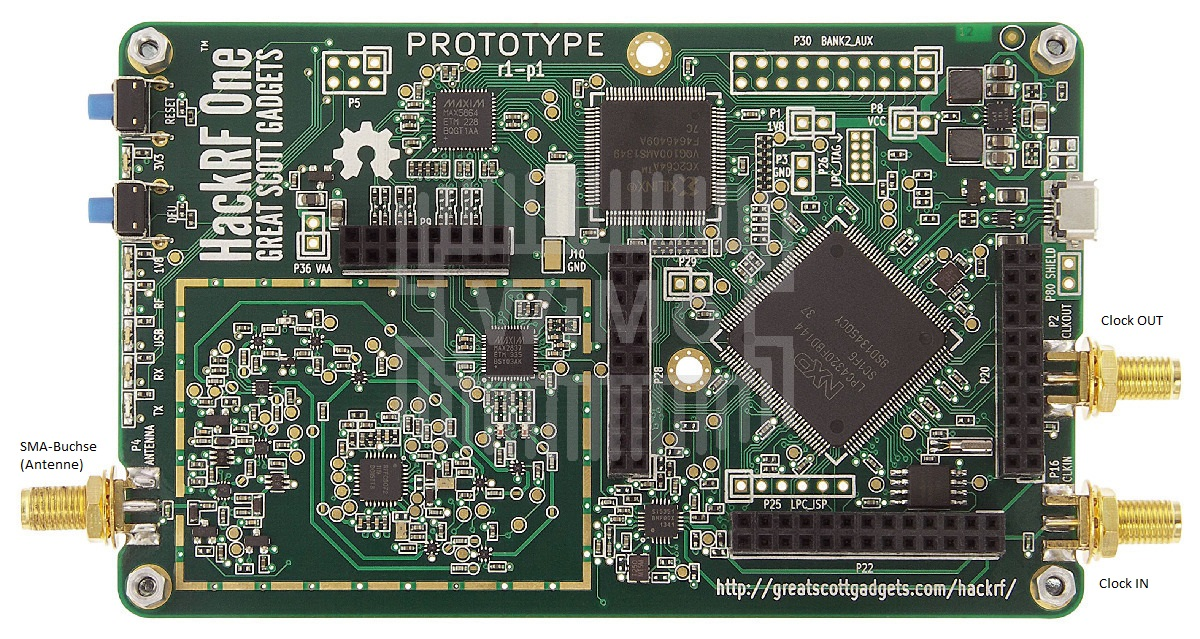
\includegraphics[width=0.75\textwidth]{HackRFOne.png}
	\caption[Hack RF ONE Platine]{Hack RF ONE Platine. Quelle: \cite{wimo:2018}} 
	\label{HackRFOne}
\end{figure}

Der Hack RF One deckt einen weiten Frequenzbereich von 1 bis 6000 MHz (6 GHz) ab, und erfasst damit sehr viele Frequenzbänder für kommerzielle, experimentelle und Amateurfunk-Anwendungen. Die Hardware bietet eine maximale Abtastrate des Signales von 20MS/s, dadurch werden Messungen und Experimente auch mit breitbandigen Signalen wie DECT, WFM oder WLAN möglich, jedoch nur halbduplex. Der AD-Wandler arbeitet mit 8 Bit Datenbreite und erreicht somit einen theoretischen Dynamikbereich von 48dB. Die digitalisierten I/Q Daten werden auf einem nachgeschalteten CPLD weiterverarbeitet und über den integrierten ARM-Prozessor per USB ausgegeben. Die gesamte Schaltung des HackRF Boards ist sehr stromsparend ausgelegt, sie wird komplett über USB versorgt. Die Platine hat eine Mikro-B USB Buchse. Abschließend lässt sich sagen, dass die oben genannten Gründe für eine optimal Nutzung dieses Gerätes sprechen \cite{wimo:2018}.\\

\begin{table}[ht]
	\centering
	\begin{tabular}{c|c}
		Modellbezeichnung & HackRF One  \\
		\hline
		Hersteller & Great Scott Gadgets\\ 
		\hline 
		Bandbreite & 20 MHz \\ 
		\hline 
		Dynamikumfang & 48 dB \\ %http://www.dolstra.nl/Ham-radio/SDR_Tranceivers/HackRF%20One%20SDR/HackRF%20One%20SDR.htm
		\hline 
		Abtastrate & \( 20 \times 10^{6} \) Hz \\ 
		\hline 
		Preis in \euro &  300 \euro\\ 
		\hline 
		Installationsart & Mobil \\ 
		\hline 
		RX/TX & RX/TX halb-duplex \\ 
	\end{tabular} 
	\caption{Produktinformationen des HackRF One}
\end{table}

Abschließend lässt sich das ein eindeutiges Ergebnis zu Stande kam, da die gewünschten Anforderungen nur durch den HackRF One gegeben sind. Was die Entscheidung, ein geeignetes SDR-Gerät deutliche simpler gestaltete.\\

Technisch realisiert ist das Frontend des HackRF One durch einen Qorvo RFFC5072 Synthesizer mit einem integrierten 6 GHz RF Mixer \cite{qorvo}.
Die Verarbeitung im Basisband bzw. in einer Zwischenfrequenz erfolgt durch einen MAX2837 Transceiver von Maxim Integrated \cite{max2837}, gefolgt von einem AD-/DA- Wandler der gleichen Firma \cite{max5864}, der das Empfangene Signal digitalisiert oder das zu sendende Signal in die analoge Domäne überführt.
\begin{figure}[H]
	\centering
	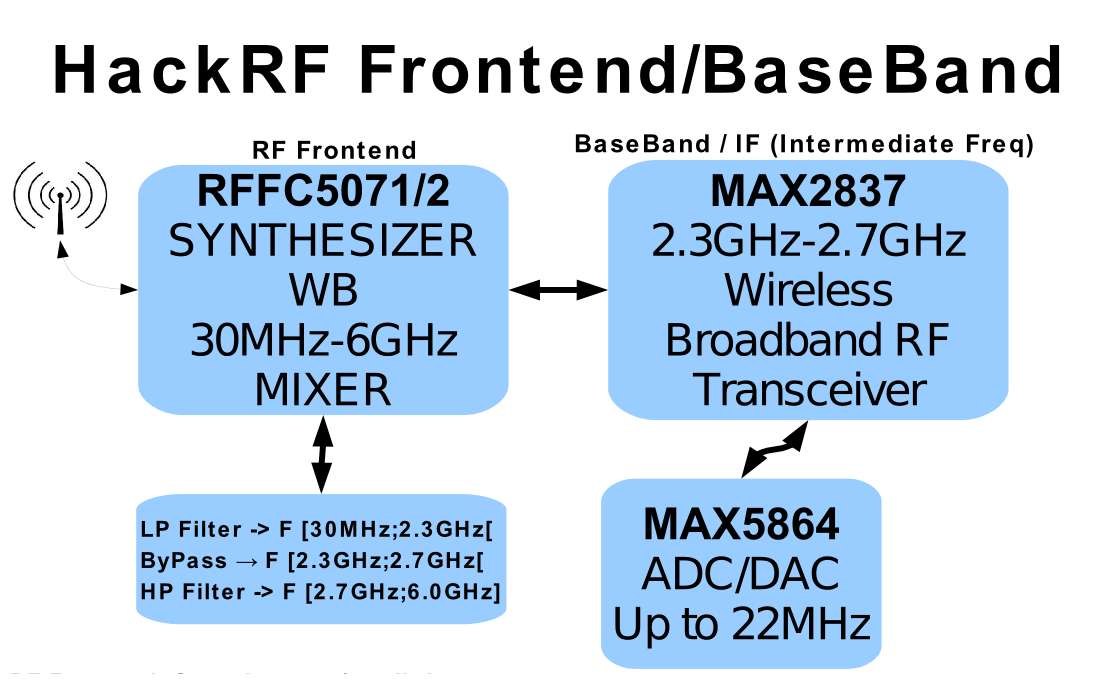
\includegraphics[width=0.7\textwidth]{hackrf-blockdiagram-frontend-baseband.png}
	\caption[Hack RF One Frontend/Baseband]{Hack RF One Frontend/Baseband. Quelle: \cite{hackrf-wiki:2016}} 
	\label{HackRFOne-Blockschaltbild}
\end{figure}

\newpage
\section{Aufbau/Entwurf}
Zu Beginn der praktischen Arbeit, wird der technische Versuchsaufbau beschrieben. Mit einer Skizze soll der Aufbau der Aufgabe detaillierte dargestellt werden. Wie in der Abbildung \ref{Technischer Aufbau} angezeigt, wird der Computer über den \ac{USB}-Anschluss mit dem HackRF One verbunden. Darüber bezieht das SDR-Gerät seine notwendige Spannungsversorgung von 5 Volt.\\
Die gegenüberliegende Seite befasst sich mit der Inbetriebnahme der ausgewählten Antenne. Diese hat einen N-Buchsen Anschluss und wird an den HackRF One angeschlossen dieser besitzt jedoch nur einen SMA-Anschluss. Dämpfung wird bei diesem Aufbau nicht berücksichtigt, da das Antennenkabel nur 10 Meter beträgt. Somit können die Geräte miteinander Kommunizieren und die empfangen Daten der Antenne bis hin zum Computer übertragen werden.  
\begin{figure}[H]
	\centering
	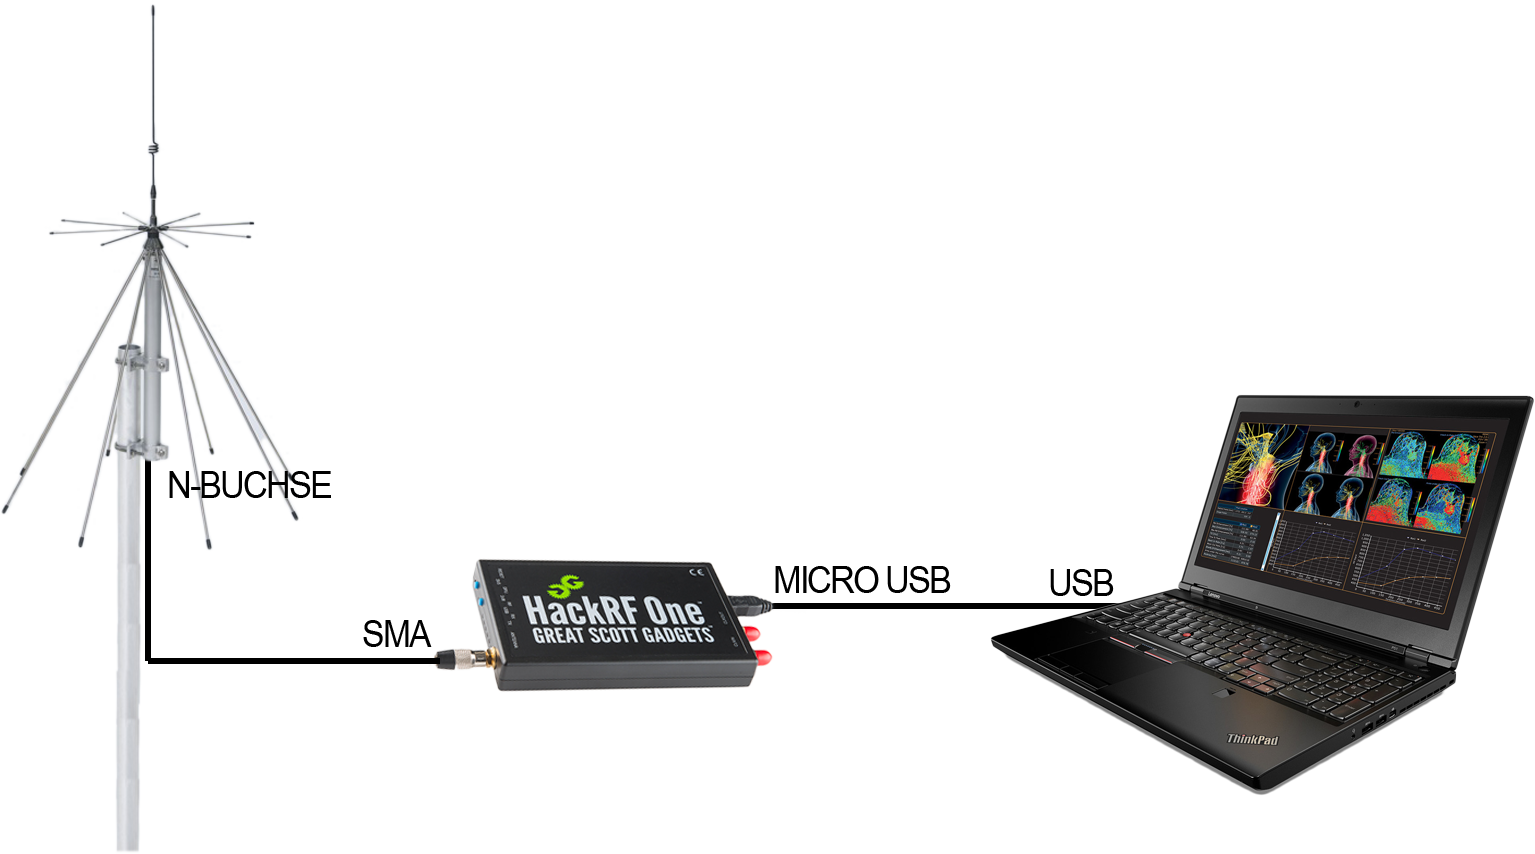
\includegraphics[width=1.0\textwidth]{TechnischerAufbau.png}
	\caption[Technischer Aufbau]{Technischer Aufbau} 
	\label{Technischer Aufbau}
\end{figure}

\newpage
\section{Spektralanalyse der Dezimeterwelle}
Die Abbildung \ref{spektralanalyse} zeigt das komplette Spektrum der Dezimeterwelle. Dabei wird erkannt welche Anwendungen in diesem Frequenzbereich liegen. Um eine solche Übersicht zu erschaffen, musste ein Interator über den Frequenzbereich genutzt werden. Der HackRF One bietet einen sogenannten Sweep Mode. Nach Installation und Inbetriebnahme dieses Modus konnte ein kompletter Bereich innerhalb von Sekunden gescannt werden. Die unten gezeigt Abbildung zeigt das komplette Spektrum der Dezimeterwelle mit den empfangenen Signalen auf den jeweiligen Frequenzen. Somit konnte eine Übersicht erstellt werden, auf welchen Frequenzen ein Signal empfangen wurde.\\

Wie sehr gut zu erkennen liegen viele und starke Signale in den Frequenzbereich 443 Mhz, 868 Mhz, 900 Mhz (GSM 900) und 1,2 GHz (GPS) weitere lokale Maxima der Kurve liegen bei 1,8 GHz - 2,2 GHz (Mobiler Landesfunkdienst UMTS) und 2,4 GHz (WLAN, Bluetooth)
\begin{figure}[H]
	\centering
	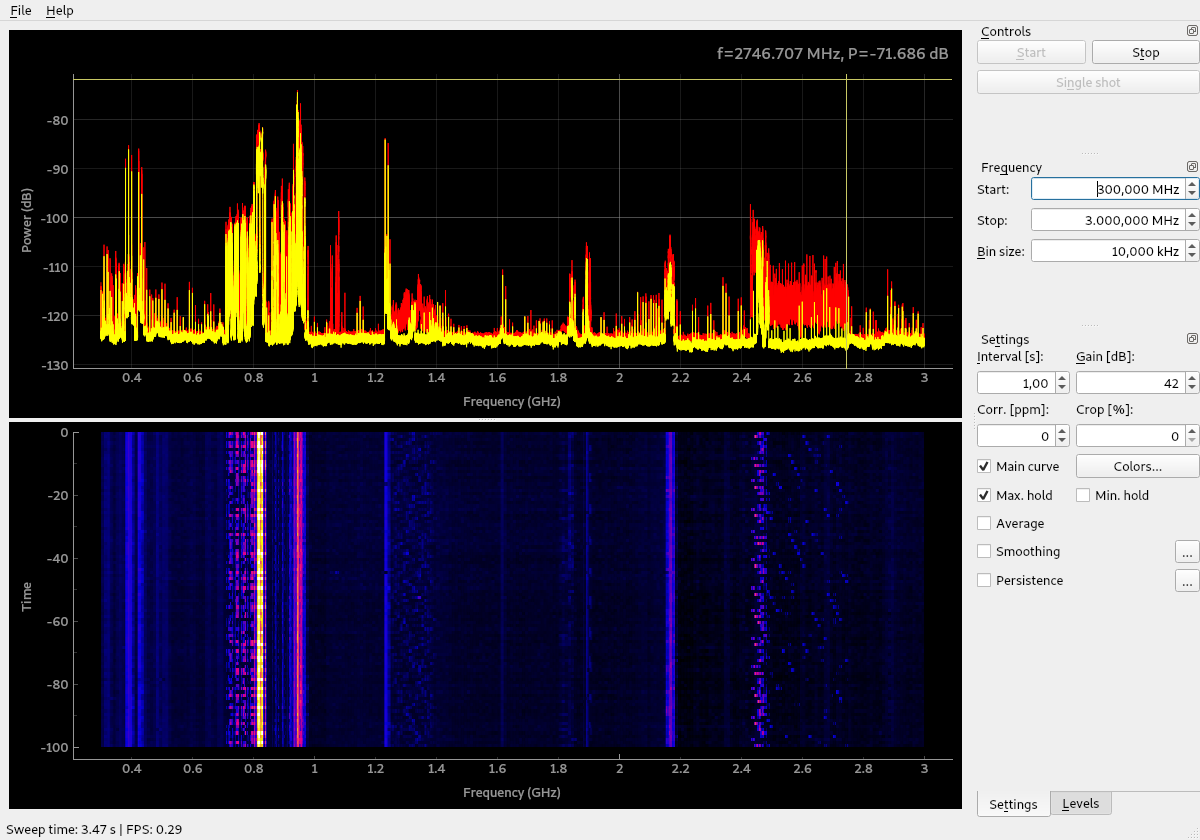
\includegraphics[width=\textwidth]{spektrum.png}
	\caption[Spektralanalyse der Dezimeterwelle]{Spektralanalyse der Dezimeterwelle. Quelle: Eigene Darstellung} 
	\label{spektralanalyse}
\end{figure}
